\documentclass[10pt]{article}
\usepackage{icmlko}

\icmlmeta{IP 파운데이션 월드모델}{296}{열여섯 행은 이득이 아니라 흔들림을 준다}{학습 문턱을 40에서 15로 내리는 갈래를 예측을 먼저 적고 닫았다 --- 청력 법칙은 이득을 못 맞혔고 대신 흔들림을 맞혔다}

\begin{document}

\twocolumn[
\icmlheader

\begin{abstract}
노트 295가 ``검출 문턱은 유보 행 수가 정한다''로 끝났다. 오늘 축을 열 개
넘게 더했고 \textbf{행은 한 번도 안 더했다.} 그래서 먼저 \textbf{어디서 행을
잃는지} 셌다 --- 유보 2,675행 중 \textbf{2,669행이 채점된다.} 잃는 것은 만화
6행(\texttt{pooled} 의 20행 최소)뿐이고, 게임에서 빠지는 43행은 노트 210이
\emph{의도해서} 뺀 것이다(긁은 날 기준 30일이 안 지난 2026년 출시작 ---
``30일 리뷰''가 아니다). \textbf{되찾을 행이 없다.} 대신 사실 하나가 드러났다
--- \texttt{MIN\_TRAIN} 은 \textbf{채점 행을 안 줄인다.} 적합 대상만 고를 뿐,
학습이 모자란 도메인도 유보 행은 그대로 채점된다. 그래서 오래 열려 있던
``문턱 40$\to$15'' 갈래는 \textbf{팝업의 학습 16행이 적합에 들어가느냐}
하나로 좁혀진다. \textbf{재기 전에 예측을 적었다}(노트 281의 청력 법칙:
나무는 \texttt{min\_samples\_leaf}${+}$2 행이 있어야 도메인 전용으로 가른다).
F18/F8 은 청력 22 라 16행으로는 못 가르고, 선형 넷은 청력 0 이라 쓸 수 있다
--- \textbf{나무는 안 움직이고 선형은 움직여야 한다.} 쟀다.
\textbf{여덟 정식화 전부 안 움직였다} --- 팝업 $|t|$ 가 0.12$\sim$0.88, 판은
전부 미결정 띠 안. 예측의 가르는 절반이 \textbf{틀렸다.} 그런데 청력이
\emph{다른 것}을 맞혔다: 팝업 \textbf{짝SE 가 무리별로 여덟 배} 갈린다(나무
0.023$\sim$0.049 · 선형 0.004$\sim$0.006), 그리고 청력 400인 F10 과
Procrustes 는 \textbf{정확히 0.0000} 이다. \textbf{청력은 이득이 아니라
흔들림을 예측한다.} 덤으로 챔피언이 지금 \texttt{t15} 에서 도는데
\textbf{40 이 $+$0.0032 낫다}(짝SE 0.0025 · $t{=}{-}1.24$ · 문턱 0.0051) ---
못 가른다. \textbf{문턱은 아무것도 안 벌고 있었다.}
\end{abstract}
]

\section{먼저 행을 셌다}

노트 274가 검출 문턱을 2$\times$짝SE 로 놓았고 노트 295가 그 짝SE 를
\textbf{유보 행 수}가 정한다는 것을 하네스에서 다시 확인했다. 오늘 하루
축을 열 개 넘게 더했는데 \textbf{행은 한 번도 안 더했다.} 잃고 있는지 셌다.

\begin{center}\footnotesize
\begin{tabular}{lrrrr}
\hline
도메인 & 행 & 학습 & 유보 & 채점 \\
\hline
웹툰 & 2,817 & 2,106 & 711 & 711 \\
세계애니 & 2,948 & 2,648 & 300 & 300 \\
애니 & 2,073 & 1,467 & 606 & 606 \\
모바일 & 2,000 & 1,559 & 441 & 441 \\
만화 & 1,789 & 1,783 & 6 & \textbf{0} \\
게임 & 482 & 259 & 180 & 180 \\
펀딩 & 400 & 320 & 80 & 80 \\
도서 & 243 & 80 & 163 & 163 \\
시장팝업 & 205 & 101 & 104 & 104 \\
아이돌 & 81 & 54 & 25 & 25 \\
팝업 & 75 & 16 & 59 & 59 \\
\hline
\textbf{합} & 13,113 & & \textbf{2,675} & \textbf{2,669} \\
\hline
\end{tabular}
\end{center}

\textbf{잃는 것은 만화 6행뿐}이고 그건 \texttt{pooled} 이 20행 미만을 안
채점하기 때문이다. 게임이 223 이 아니라 180 인 것은 노트 210이 \emph{의도해서}
뺀 43행 --- 긁은 날 기준 30일이 안 지난 2026년 출시작이라 ``30일 리뷰''라는
측정이 아직 성립하지 않는다. \textbf{되찾을 행이 없다.}

\paragraph{그런데 셋다가 다른 것을 봤다} \texttt{MIN\_TRAIN} 은
\textbf{적합 대상 도메인}만 고른다. 학습이 모자란 도메인도 \textbf{유보 행은
그대로 채점된다} --- 다른 도메인에서 배운 것으로 예측하는 것이 이 판의
설계이기 때문이다. 팝업은 학습 16행으로 문턱 40에 걸려 있지만 \textbf{유보
59행이 지금도 전부 채점되고 있다.}

그래서 오래 열려 있던 ``문턱 40$\to$15'' 갈래가 한 문장으로 좁혀진다:
\textbf{팝업의 학습 16행이 적합에 들어가느냐.} 나머지 열 도메인은 학습이
54행(아이돌) 이상이라 문턱이 40이든 15든 같다.

\section{재기 전에 예측을 적었다}

\begin{figure*}[t]
\centering
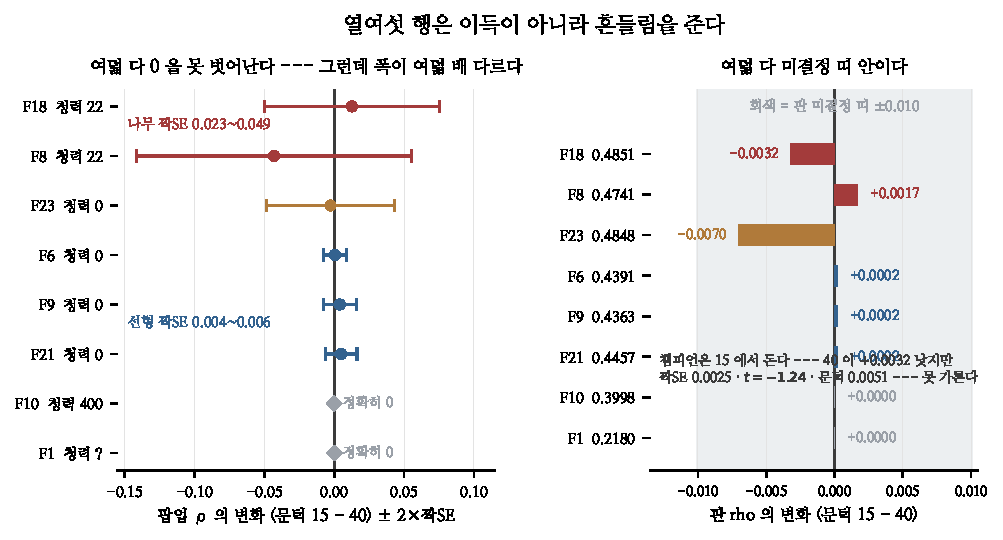
\includegraphics[width=\textwidth]{figs/sixteen.pdf}
\caption{왼쪽 --- 문턱을 15로 내렸을 때 팝업 $\rho$ 의 변화($\pm$2$\times$짝SE,
부트스트랩 400). 오른쪽 --- 같은 변화의 판 $\rho$.}
\end{figure*}

노트 281의 청력 법칙: 나무 정식화가 \emph{도메인 전용}으로 가르려면 학습
관측 행이 \texttt{min\_samples\_leaf}${+}$2 이상이어야 한다.

\begin{center}\footnotesize
\begin{tabular}{lrl}
\hline
정식화 & 청력 & 팝업 16행으로 \\
\hline
F18 · F8 & 22 & \textbf{못 가른다} $\to$ 안 움직여야 \\
F6 · F9 · F21 · F23 & 0 & 쓸 수 있다 $\to$ 움직일 수도 \\
F10 & 400 & 확실히 안 움직인다 \\
\hline
\end{tabular}
\end{center}

이것을 \texttt{data/lab/preregister\_minTrain.json} 에 적고 나서 쟀다.
미리 적은 실패도 함께: ``선형 넷도 전부 안 움직이면 16행은 어느 정식화에도
너무 적다는 것이고, 청력 법칙은 이 시험에서 아무것도 안 갈랐다.''

\section{가르는 절반이 틀렸다}

\begin{center}\footnotesize
\begin{tabular}{lrrrrr}
\hline
정식화 & 청력 & 판 40 & 판 15 & 팝업 $\Delta$ & $t$ \\
\hline
F18 & 22 & 0.4851 & 0.4819 & $+$0.0127 & 0.41 \\
F8 & 22 & 0.4741 & 0.4758 & $-$0.0431 & $-$0.88 \\
F23 & 0 & 0.4848 & 0.4778 & $-$0.0027 & $-$0.12 \\
F6 & 0 & 0.4391 & 0.4393 & $+$0.0005 & 0.12 \\
F9 & 0 & 0.4363 & 0.4365 & $+$0.0040 & 0.68 \\
F21 & 0 & 0.4457 & 0.4459 & $+$0.0049 & 0.85 \\
F10 & 400 & 0.3998 & 0.3998 & \textbf{0.0000} & --- \\
F1 & ? & 0.2180 & 0.2180 & \textbf{0.0000} & --- \\
\hline
\end{tabular}
\end{center}

\textbf{여덟 다 안 움직였다.} 팝업 $|t|$ 가 전부 1 아래고, 판은 여덟 다
미결정 띠($\pm$0.010) 안이다. \textbf{미리 적은 대로 이것은 실패다} ---
청력 법칙이 나무와 선형을 갈라 놓았는데 자료는 안 갈렸다.

\paragraph{그런데 청력이 다른 것을 맞혔다} 이득이 아니라 \textbf{흔들림}이다.

\begin{center}\footnotesize
\begin{tabular}{lrl}
\hline
무리 & 팝업 짝SE & \\
\hline
나무(F18 · F8 · F23) & 0.023$\sim$0.049 & \textbf{여덟 배} \\
선형(F6 · F9 · F21) & 0.004$\sim$0.006 & \\
도메인별(F10 · F1) & \textbf{0.0000} & 안 쓴다 \\
\hline
\end{tabular}
\end{center}

\textbf{같은 16행이 선형에는 작고 한 방향인 변화를, 나무에는 크고 방향 없는
변화를 준다.} 선형 셋은 $+$0.0005 · $+$0.0040 · $+$0.0049 로 \textbf{셋 다
양수}지만 짝SE 안이고, 나무 셋은 $+$0.0127 · $-$0.0431 · $-$0.0027 로
\textbf{부호가 흩어진다.} 그리고 청력 400인 F10 과 도메인별 PCA 를 쓰는
Procrustes 는 \textbf{정확히 0.0000} --- 16행을 아예 안 쓴다는 뜻이고,
그건 청력 법칙이 정확히 예측한 것이다.

\textbf{청력 문턱 아래의 행은 사라지는 게 아니라 잡음이 된다.}

\section{그리고 챔피언의 문턱이 아무것도 안 벌고 있었다}

챔피언 이름이 \texttt{F18\_bagboost@trendcalwikitag$\cdot$t15} 다. 뒤의
\texttt{t15} 가 \texttt{MIN\_TRAIN}${=}$15 이다 --- \textbf{챔피언은 이미
15에서 돈다.} 그런데

\begin{center}\small
\begin{tabular}{lr}
\hline
판 40 & 0.4851 \\
판 15 & 0.4819 \\
\hline
차 & \textbf{$-$0.0032} \\
짝SE & 0.0025 \\
$t$ & $-$1.24 \\
검출 문턱 & 0.0051 \\
\hline
\end{tabular}
\end{center}

\textbf{못 가른다.} 15가 40보다 낫다는 증거도 없고 나쁘다는 증거도 없다.
바꿀 이유가 없으므로 \textbf{그대로 둔다} --- 다만 이제 그것이 ``측정해서
고른 값''이 아니라 \textbf{``측정해 보니 아무래도 좋은 값''}이라는 것을 안다.

\paragraph{남은 것}
\begin{center}\small
\begin{tabular}{ll}
\hline
갈래 & 왜 \\
\hline
하네스 셋 넓히기 & 돌고 있다(+57건 · 사전 등록) \\
팝업 학습 행 늘리기 & 16$\to$22 면 F18 이 듣는다 \\
청력을 흔들림으로 & 이득 말고 짝SE 를 예측한다 \\
lab 회사 축 & 노트 294의 $+$0.0040 을 남길지 \\
\hline
\end{tabular}
\end{center}

\paragraph{규약} \textbf{예측을 적고 재면 틀려도 남는 게 있다.} 이번 예측의
가르는 절반(나무 대 선형)은 틀렸는데, 틀렸다는 것을 알아서 \emph{맞은
절반}(정확히 0.0000 · 짝SE 여덟 배)을 볼 수 있었다. 적어 두지 않았으면
``여덟 다 안 움직였다''로 끝났을 것이다. 그리고 \textbf{설정값이 무엇을 버는지
한 번은 재라} --- 챔피언의 \texttt{t15} 는 판을 0.0032 만큼 \emph{잃고}
있었고, 문턱 아래라 아무도 못 봤다.

\end{document}
